\documentclass{article}
%\usepackage[a4paper, total={6in, 8in}]{geometry}
\usepackage{graphicx}
\usepackage{geometry}
\usepackage{float}
\geometry{
	a4paper,
	total={210mm,297mm},
	left=20mm,
	right=20mm,
	top=-2mm,
	bottom=2mm,
}
%\usepackage[margin=0.5in]{geometry}

\usepackage{amsmath,amssymb}
\usepackage{ifpdf}
%\usepackage{cite}
\usepackage{algorithmic}
\usepackage{array}
\usepackage{mdwmath}
\usepackage{pdfpages}
\usepackage{mdwtab}
\usepackage{eqparbox}
\usepackage{cite}
%\onecolumn
%\input{psfig}
\usepackage{color}
\usepackage{graphicx}
\setlength{\textheight}{23.5cm} \setlength{\topmargin}{-1.05cm}
\setlength{\textwidth}{6.5in} \setlength{\oddsidemargin}{-0.5cm}
\renewcommand{\baselinestretch}{1}
\pagenumbering{arabic}
\usepackage{ragged2e}
\renewcommand{\baselinestretch}{1.5}

\begin{document}
	
	\textbf{
		\begin{center}
			{
				\large{School of Engineering and Applied Science (SEAS), Ahmedabad University}\vspace{4mm}
			}
		\end{center}
		%
		\begin{center}
			\large{B.Tech(CSE) Semester IV: Probability and Stochastic Processes (MAT 277) }\\ \vspace{3mm}
		\end{center}
	}
	\begin{itemize}
		\item Group No : \textbf{SB16} 
		\item Name (Roll No) :Homak Patel(AU1940042) , Hirmay Sandesara(AU1940265) , Henil Shah(AU1940205) , Shubham Jain (AU1940315) , Gaurav Bajaj(AU1940169) , Devanshu Magiawala(AU1940190) %\item Roll no: s1749002 (Ph.d)
		%\item Associated with Project: DST-UKIERI
		\item Project Title: \underline{\textbf{Modeling the Natural History \& Detection of Lung Cancer Based on Smoking Behavior
		}}
	    \item Base Article : X. Chen, M. Foy, M. Kimmel, and O. Y. Gorlova, “Modeling the Natural History and Detection of Lung Cancer Based on Smoking Behavior,” PLoS ONE, vol. 9, no. 4, 2014.
		
	\end{itemize} 
    \section {Justification And Modelling Of Uncertainities}
	The age of the person during the formation of primary tumor and initiation of nodal and distant metastasis is considered as one of the most uncertain and important factors during the treatment of lung cancer. With a proper idea about the age, a very good prognosis could be achieved. Through the carcinogenesis model based upon two-stage clonal expansion models (Venzon and Moolgavkar), one is able to predict this very important factor during the instant of tumor initiation. \\
	
	Even the progression of lung cancer with time is also a very uncertain event, before modelling these uncertainties one has to make certain assumptions. The summarised version of these assumptions which also mention the concepts used by us are,
	Parameter $\lambda$ is described as the time for the tumor to grow double to its original size. Therefore, the parameter $\lambda$ (which is the growth rate factor) follows a gamma distribution's probability density function, with scale and shape parameters $\theta $ { and } $ K$. The cell activity of a tumor can be described by parameter $\alpha$, to which the growth rate parameter $\lambda$ is directly proportional. \\
	
	Therefore $\lambda = \epsilon_1 * \alpha$ (In this equation, $\epsilon_1 $ is taken as constant).The cell detachment rate, $\beta$, is also proportional to $\alpha$, $\beta = \epsilon_2 * \alpha$ (Here also,
	$\epsilon_2$ is constant). Thus, $\beta = \frac{\epsilon_2}{\epsilon_1} \lambda$, where $\frac{\epsilon_2}{\epsilon_1} = \xi$ can be assumed as the parameter which describes the relation existing between $\beta \text{ and } \lambda$. In a scenario where
	the volume (represented by parameter S) of tumor grows exponentially, $S=e^{\lambda * t}$ , the total number of detached cells before time $\tau_0$ is $e^{\xi \lambda \tau_0} = S_0^{\xi}$; we assume $0<\xi<1$, the interpretation of which is that cells always detach from the primary tumor but not all tumor cells will detach. Additionally we have also calculated the PDFs through differentiation of the corresponding CDFs.\\
	
	Cancer detection is considered a competing process of detecting primary tumor or nodal or distant metastases. The author developed the model for Cancer Detection through rigorous calculations with exponential growth of tumors as logical assumption. The CDF of detection of primary tumor, nodal and distant metastasis through estimations are denoted as Dp(s), Dn(s) and Dm(s).\\
	
	In this estimation section of research, the CDF of primary tumor size, nodal and distant metastasis are defined with the help of some parameters. \\ 
	\begin{align}
			D_{p} ( s_{p}) = 1 -  e^{-\frac{\alpha}{2} s_{p}^{2} -  w_{0} s_{p}} \\
            D_{n} ( s_{n}) = 1 -  e^{-\frac{\alpha}{2} s_{n}^{2} -  w_{1} s_{n}}
	\end{align}
   
	As mentioned in File S1 (Simulation Procedure file attached with research paper), we generated a random number for each patient based upon uniform distribution on (0,1) and checked if it were less than or equal to Dp(sp) or Dn(sn). Here, sp and sn are the size of the primary tumor and nodal metastasis. If it were, it was included in the lung cancer detection population. The process is repeated until the time of his death.\\

	
	As SEER 1988-99 and SEER 2000-03 were the only data sets that were available to us, some parameters and specifications that are available in the dataset SEER 2004-08, which was also used in research paper, were not used in the modelling that we have simulated and also results into some inaccuracy as some the estimated parameters were also calculated on the basis of data available from SEER 2004-08 as mentioned in the simulation file S1 of the research article. Moreover, there were no patients staged at TNM staging M1, and so, some of the corresponding graphs could not be drawn.\\
	
	
	
	\subsection{Tumor Growth And Metastasis Modelling}
	
	According to given paper, we have identified and analysed the various assumptions which were mentioned in the modelling of tumor growth and metastasis.By identifying the various assumptions, we were able to simplify our problem and get a better intution on ways to approach problem and provide appropriate solutions. This assumptions were mentioned in Justification section\\
	
	Below are the equations of CDF in terms of size of tumor ,
	$$F_n(s) = 1- e^{- \frac{\mu_n}{\xi +1} * S(\xi +1)}$$
	$$F_m(s) = 1- e^{- \frac{\mu_m}{\xi +1} * S(\xi +1)}$$\\
	Therefore, the corresponding probability density functions to these cummulative distribution functions come out to be, \\ 
	
	$$f_n(\tau) = \int f_n(\tau,\lambda)* \gamma(\lambda|k,\theta)d\lambda$$
	$$f_m(\tau) = \int f_m(\tau,\lambda)* \gamma(\lambda|k,\theta)d\lambda$$
	$$f_{n1m0}(\tau) = \int (f_n(\tau,\lambda) - f_m(\tau,\lambda)) * \gamma(\lambda|k,\theta)d\lambda$$
	
	Here, $f_n(\tau)$ is the gennerated p.d.f for nodal metastasis and  $f_m(\tau)$ is the p.d.f of distant metastasis whereas $f_{n1m0}(\tau)$ is the p.d.f of only nodal metastasis (without having distant metastasis)\\
	

	
	We calculated the above PDF's using inverse laplace transform, as the computed cummulative density function seemed more closely to laplace distribution. Hence, we then tried to apply inverse laplace transform to given c.d.f in order to transform the given c.d.f from being c.d.f in terms of s (size) to in terms of time t, but here also, it wasn't able to calculate it due to fractional power (as the power of S was 1.01).\\
	
	
	%\item Explain the probabilistic model used to solve the problem
	
	
	\section{Changes in Coding Part}
	
	\begin{enumerate}
		\item Calculation of the probability density functions given in the paper were evaluated using an alternate method. In the paper they have given the PDFs in the integral form which are quite complex and also need additional data. Therefore, we incorporated Inverse Laplace Transformation of the given cdfs and on differentiating them we’re able to get respective PDFs.
		
		\item The code provided to us had a lower amount and less details as compared to what authors have used in the research paper. So,we extracted data from the given .xlsx files of SEER i.e. SEER 1988-99 and SEER data 2000-03 with help of xlrd libraries of python.
		\item Analysed the tumor sizes of data in both .xlsx files and computed the frequency and probability distribution based on the type of modelling.
		\item Implemented the probability distribution of tumor size ranges after analyzing data in the .xlsx file of SEER 2000-03 and using xlrd library of python for reproducing graph-2(A) of research paper.
		\item Implemented the calculation of cdf function of tumor size with the help of sympy library of python and calculated the probability distribution of different tumor size ranges that can be used in reproducing the graph-2(A) of research paper.
		For reproducing graph-2(B), analyzed data from SEER 2000-03 and used xlrd python library for importing values and plotting the SEER 2000-03 data.
		
		\item Calculated the cdf of primary tumor detection and nodal metastasis of tumor size and used that for the modelling of data which is used to plot the fitted model’s frequency distribution for SEER 2000-03 data.
		
		\item Implemented the probability distribution of tumor size ranges of stage N0M0 after analyzing data in the .xlsx file of SEER 1988-99 and using xlrd library of python for reproducing graph-3(A) of research paper.
		
	   	\item Calculated the cdf of primary tumor and nodal metastasis of tumor size for SEER 1988-99 data for different tumor ranges of stage N0M0 and used that for the modelling of data which is used to plot the simulated model’s frequency distribution for SEER 1988-99 data in graph-3(A) of research paper.
		
		\item Implemented the probability distribution of tumor size ranges of stage N1M0 after analyzing data in the .xlsx file of SEER 1988-99 and using xlrd library of python for reproducing graph-3(B) of research paper.
		
		\item Calculated the cdf of primary tumor and nodal metastasis of tumor size for SEER 1988-99 data for different tumor ranges of stage N1M0 data and used that for the modelling of data which is used to plot the simulated model’s  frequency distribution for SEER 1988-99 data in graph-3(B) of research paper.
		
		\item We have implemented different types of modelling like Logistic regression classification, SVM (Support Vector Machine) classification ,Naive bayes classification , Decision tree classification , Random forest classification with the help of Machine Learning because we want to see which model is the optimal for our given database.
		
	\end{enumerate}
	\pagebreak
	
	
	\section{Contribution of team members}	
	\subsection{Technical contribution of all team members }
\begin{table}[H]
	\centering
	\begin{tabular}{|l|l|l|l|l|l|l|} 
		\hline
		Task   & \begin{tabular}[c]{@{}l@{}}Homak \\ Patel\end{tabular}                              & \begin{tabular}[c]{@{}l@{}}Henil \\ Shah\end{tabular}                      & \begin{tabular}[c]{@{}l@{}}Hirmay \\ Sandesara\end{tabular}                      & \begin{tabular}[c]{@{}l@{}}Shubham\\ Jain\end{tabular}                            & \begin{tabular}[c]{@{}l@{}}Gaurav\\ Bajaj\end{tabular}                              & \begin{tabular}[c]{@{}l@{}}Devanshu \\ Magiawala\end{tabular}  \\ 
		\hline
		Task-1 & \begin{tabular}[c]{@{}l@{}}Analytical \\ Research\end{tabular}                      & \begin{tabular}[c]{@{}l@{}}Mathematical\\ Analysis\end{tabular}            & \begin{tabular}[c]{@{}l@{}}Mathematical\\ Analysis\end{tabular}                  & \begin{tabular}[c]{@{}l@{}}Data \\ Analysis\end{tabular}                          & \begin{tabular}[c]{@{}l@{}}Data \\ Analysis\end{tabular}                            & -                                                              \\ 
		\hline
		Task-2 & \begin{tabular}[c]{@{}l@{}}ML Model\\ Training And \\ Testing\end{tabular}          & \begin{tabular}[c]{@{}l@{}}ML Model\\ Training And \\ Testing\end{tabular} & \begin{tabular}[c]{@{}l@{}}Biological \\ Analysis And \\ Research\end{tabular}   & \begin{tabular}[c]{@{}l@{}}Existing Results \\ Regeneration\end{tabular}          & \begin{tabular}[c]{@{}l@{}}Existing Results \\ Regeneration\end{tabular}            & -                                                              \\ 
		\hline
		Task-3 & \begin{tabular}[c]{@{}l@{}}Mathematical\\Proofing \\ (Innovation part)\end{tabular} & \begin{tabular}[c]{@{}l@{}}Data Generation \\ (Innovation)\end{tabular}    & \begin{tabular}[c]{@{}l@{}}Coding Based\\ Simulation\\ (Innovation)\end{tabular} & \begin{tabular}[c]{@{}l@{}}Coding Based\\ Simulation \\ (Innovation)\end{tabular} & \begin{tabular}[c]{@{}l@{}}Mathematical \\Proofing\\ (Innovation Part)\end{tabular} & -                                                              \\
		\hline
	\end{tabular}
\end{table}
\linebreak

	\subsection{Non-Technical contribution of all team members}
	
	\begin{table}[H]
		\begin{tabular}{|l|l|l|l|l|l|l|}
			\hline
			Task   & \begin{tabular}[c]{@{}l@{}}Homak \\ Patel\end{tabular}                    & \begin{tabular}[c]{@{}l@{}}Henil \\ Shah\end{tabular}                              & \begin{tabular}[c]{@{}l@{}}Hirmay \\ Sandesara\end{tabular}                & \begin{tabular}[c]{@{}l@{}}Shubham\\ Jain\end{tabular}                         & \begin{tabular}[c]{@{}l@{}}Gaurav\\ Bajaj\end{tabular}                          & \begin{tabular}[c]{@{}l@{}}Devanshu \\ Magiawala\end{tabular} \\ \hline
			Task-1 & \begin{tabular}[c]{@{}l@{}}Concept \\ Map\end{tabular}                    & \begin{tabular}[c]{@{}l@{}}Concept \\ Map\end{tabular}                             & \begin{tabular}[c]{@{}l@{}}Concept \\ Map\end{tabular}                     & \begin{tabular}[c]{@{}l@{}}Concept \\ Map\end{tabular}                         & \begin{tabular}[c]{@{}l@{}}Concept \\ Map\end{tabular}                          & \begin{tabular}[c]{@{}l@{}}Concept \\ Map\end{tabular}        \\ \hline
			Task-2 & \begin{tabular}[c]{@{}l@{}}Innovation \\ Section \\ (Report)\end{tabular} & \begin{tabular}[c]{@{}l@{}}Justification\\ and Report \\ Coordination\end{tabular} & \begin{tabular}[c]{@{}l@{}}Justification \\ and \\ inferences\end{tabular} & \begin{tabular}[c]{@{}l@{}}Results '\\ and \\ Graphs\\ Extraction\end{tabular} & \begin{tabular}[c]{@{}l@{}}Results\\ and \\ Graphs\\ Extraction\end{tabular}    & -                                                             \\ \hline
			Task-3 & \begin{tabular}[c]{@{}l@{}}LATEX\\ code\end{tabular}                      & Inferences                                                                         & \begin{tabular}[c]{@{}l@{}}Report \\ Proof \\ Reading\end{tabular}         & \begin{tabular}[c]{@{}l@{}}Inferences\\ and \\ conclusions\end{tabular}        & \begin{tabular}[c]{@{}l@{}}Changes in\\ Existing\\ code\\ (Report)\end{tabular} & -                                                             \\ \hline
		\end{tabular}
	\end{table}
	\pagebreak
	\section{Innovation} 
	
	\begin{enumerate}
		
		\item \textbf{\large Introduction} 
		
		While smoking is still the leading cause of lung cancer, accounting for 80 \% to 90 \% of all cases, heredity may play a role in the disease in some cases. Lung cancer is thought to be due to a genetic predisposition in around 8\% of cases. Even though having a parent or sibling with lung cancer increases the risk, it does not guarantee that any individual will develop the disease. So, we have tried to model a relationship between “Genetic Risk” and “Lung Cancer”. So for modeling, we are using hypothesis testing in which we are trying to produce some useful inferences based on our dataset. \\ 
		
		\textbf{\large Dataset:}   
		
		The dataset that we have considered for the innovation part contains some important data like “Genetic Risk” which is calculated on a specific scale of 1-10 for different districts (with unique FIPS code). The dataset also includes the Lung Cancer incident rates of that district based on the factor of “Genetic Risk”.
		Besides the provided data we have added one more column “Status Variable” which takes only two values ‘0’ and ‘1’ depending upon the scale value of  “Genetic Risk”. As per our null hypothesis, we have assigned the value “0” to the districts which have a genetic risk factor less than 5 and we have assigned the value “1” to the districts with a genetic risk factor greater than 5. 
		\\ 
		
		
		\textbf{\large T-Test (Hypothesis Testing)} 
		
		\textbf{Null hypothesis ($H_{0}$)}: The districts with a high Genetic Risk have high lung cancer incidence rates than those with low genetic risk.\\
		
		\textbf{Alternative Hypothesis ($H_{1}$):} The districts with a high Genetic Risk have less lung cancer incidence rates than those with low genetic risk. 
		
		\textbf{\large Assumptions for T-test:} 
		
		1. Data follows a normal distribution which implies we can make a Q-Q plot.\\
		2. The variance of the 2 samples are the same which implies use the Chi-square test for a variance to show this. \\
		3. Data of a dataset used is continuous which implies that upon inspection it holds.\\
		4. We are conducting a test at a 95\% confidence interval which implies that the value of alpha is 0.05. \\ 
		
		\textbf{\large Main Steps for Calculations in simulation:} 
		
		\textbf{(1) Extracting and Reading Data from the Dataset:} \\
		The first step for the simulation is to read the .csv file of our dataset on which we want to apply our t-test. So, in the first step, we have extracted all the columns of attributes that we want to use for our testing.  
		
		\textbf{(2) Differentiating and Selecting the data depending upon the Null Hypothesis:} \\
		So, in this step, we have extracted the values depending upon our Null Hypothesis ($H_{0}$). Here we have defined two variables “gen-hi” and “gen-lo” depending upon their “status variable” values.
		\\"gen-hi" includes all the rows which have a “state variable” value of “1”.
		"gen-lo" includes all the rows which have a “state variable” value of “0”. 
		
		\textbf{(3)Plotting the Probability Plot of incident rates of “Lung Cancer” and “Status variables” depending upon High risk (gen-hi) and Low risk (gen-lo) :}
		
		In this step, we are plotting the Q-Q probability plot between incident rates of Lung Cancer in high genetic risk (gen-hi). We are also plotting the Q-Q probability plot between incident rates of Lung Cancer in low genetic risk (gen-lo). 
		
		
		\begin{figure}[htbp]
			\centerline{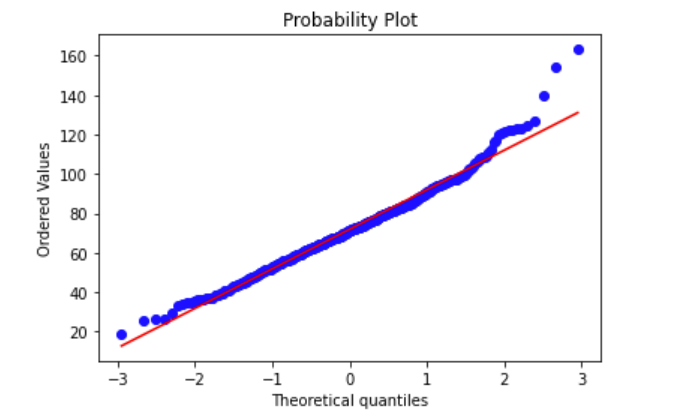
\includegraphics[scale=.5]{1.png}}
			\caption{Q-Q probability plot between incident rates of Lung Cancer in high genetic risk (gen-hi)}%
			
		\end{figure}	

		
		\textbf{(4) Calculating the Mean values and F-statistic:} \\ 
		In this step, we have calculated the mean of incident rates of lung cancer where there are high genetic risk and the mean of incident rates of lung cancer where there is low risk and also we have calculated variances and F-statistic value which can be used for deriving important inferences.  Our test statistic is var-hi/var-lo under the null hypothesis now we need to calculate the p-value. \\ 
		\textbf{(5) Calculating the p-value and t-statistic for distribution :
		} \\
		In this step, we have calculated the final p-value from other calculated values like F-statistic , dfhi and dflo. So this p-value can be used to derive our final result by comparing it with a value of alpha which is 0.05 here as we are estimating our test at a 95\% confidence interval. \\ \\ 
		\\ \\
		
		
	\end{enumerate}
	
	
	
	\section{Inferences derived from user-centric perspective.}
	
	\begin{enumerate}
		
			\item \textbf{\underline{Probability Density Function of Distant and Nodal Metastatis From the time of tumor Onset }}
			\begin{figure}[htbp]
				\centerline{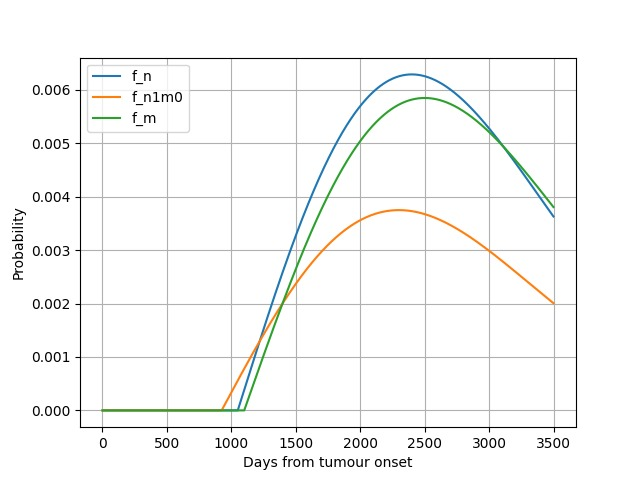
\includegraphics[scale=.35]{7.jpeg}}
				\caption{PDF Curve of  Distant and Nodal Metastatis From the time of tumor Onset }		
			\end{figure}
		
		After the process mentioned in section 1.1 we approximated these equations and computed the inverse laplace transform and then, the c.d.f obtained after inverse laplace transform is then differentiated in terms of t, and the equation that is obtained resembles more towards p.d.f of rayleigh distribution. Hence, we then concluded our probability distribution functions to be rayleigh distribution's probability distribution functions.\\
		
		Hence, the p.d.f's obtained would be \\
		$$f_n(\tau) =  14*e^ {-(t^2)/2*(1350^2)}$$
		$$f_m(\tau) = 13.5*e^{-(t^2)/2*(1400^2)} $$
		$$F_{n1m0}(\tau) =  8.5*e^ {-(t^2)/2*(1375^2)}$$
		
		\pagebreak
			
		\item \textbf{\underline{Fitting Data based upon SEER 2000-2003 lung cancer data}}
		
		\begin{figure}[H]
			\centerline{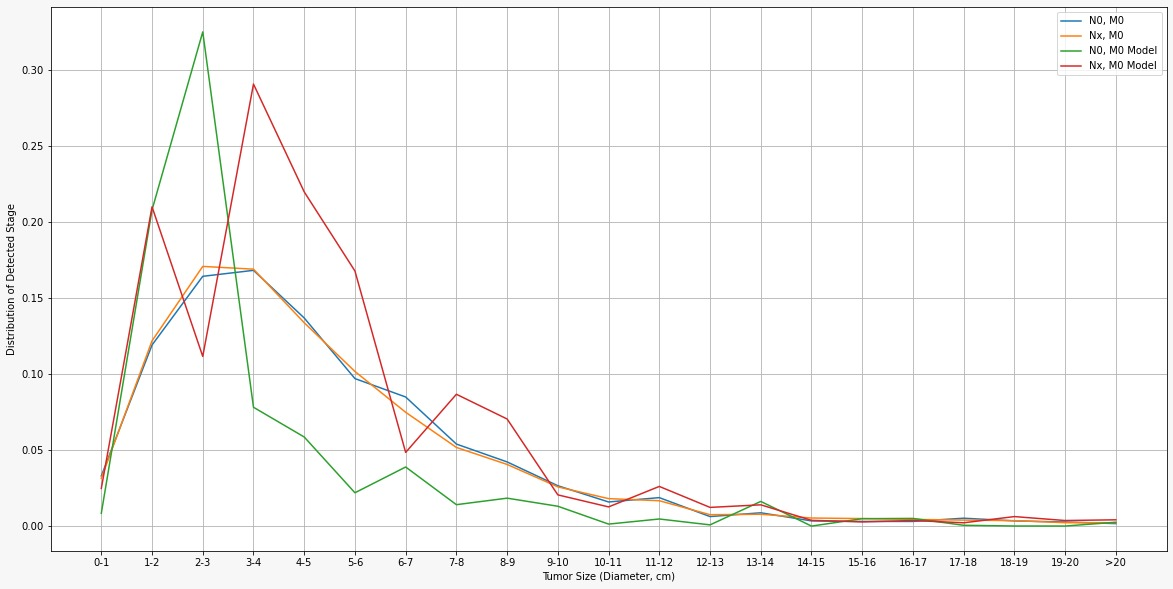
\includegraphics[scale=.25]{3.jpeg}}
			\caption{Stage Distribution Conditional On Tumor Size}		
		\end{figure}
	The graph shows the distribution of detected stages based upon the different ranges of tumor sizes. The graph shows the comparison of detected stage distribution between given data and modelled data. The SEER 2000-2003 data had records for patients belonging to either N0,M0 stage or Nx, M0 stage. There were no patients recorded that belonged to M1 stage. As per the graph, one can clearly see that at lower tumor sizes modelled data deviates slightly from the original one, but at larger tumor sizes (after 11-12 cm tumor size range), original and modelled data converges. Also, one can observe more frequent deviations in Nx,M0 modelled data as compared to N0,M0 modelled data. This shows that the model is successful in predicting original results at larger tumor sizes. The accuracy of reproducing original results could be increased in the availability of larger datasets.



	
	
	\begin{figure}[H]
		\centerline{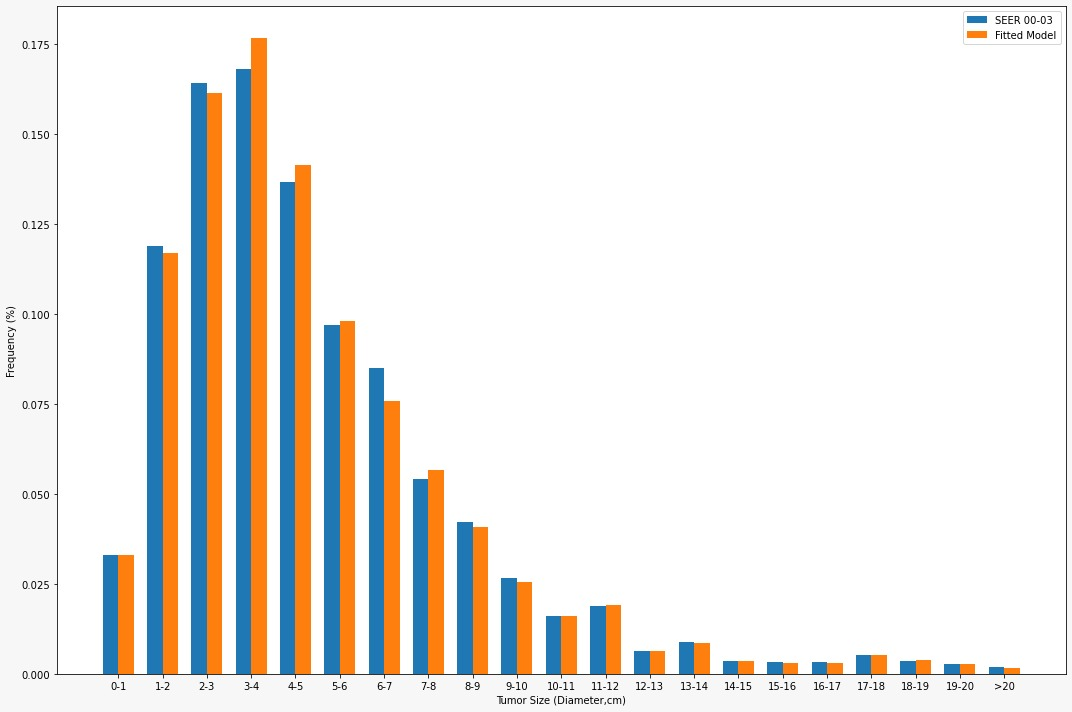
\includegraphics[scale=.35]{4.jpeg}}
		\caption{Tumor Size Distribution}		
	\end{figure}

This graph combines the characteristics of line charts of both N0,M0 and Nx,M0 patients and produces frequency distribution of patients based upon different tumor size ranges (plotted on the x-axis). The same inference can also be collected from this graph. This graph also shows the deviation of results from the given model at the initial size of the tumor. Clearly, at larger sizes of the tumor, the modelled data generates characteristics similar to the original given data. Also, for tumor sizes less than a cm, the model has correctly predicted the frequency distribution of patients.\\
	
	
	
\pagebreak	
	 
\item  \textbf{\underline{Tumor Size Distribution in Predictive Models}}

	\begin{figure}[htbp]
		\centerline{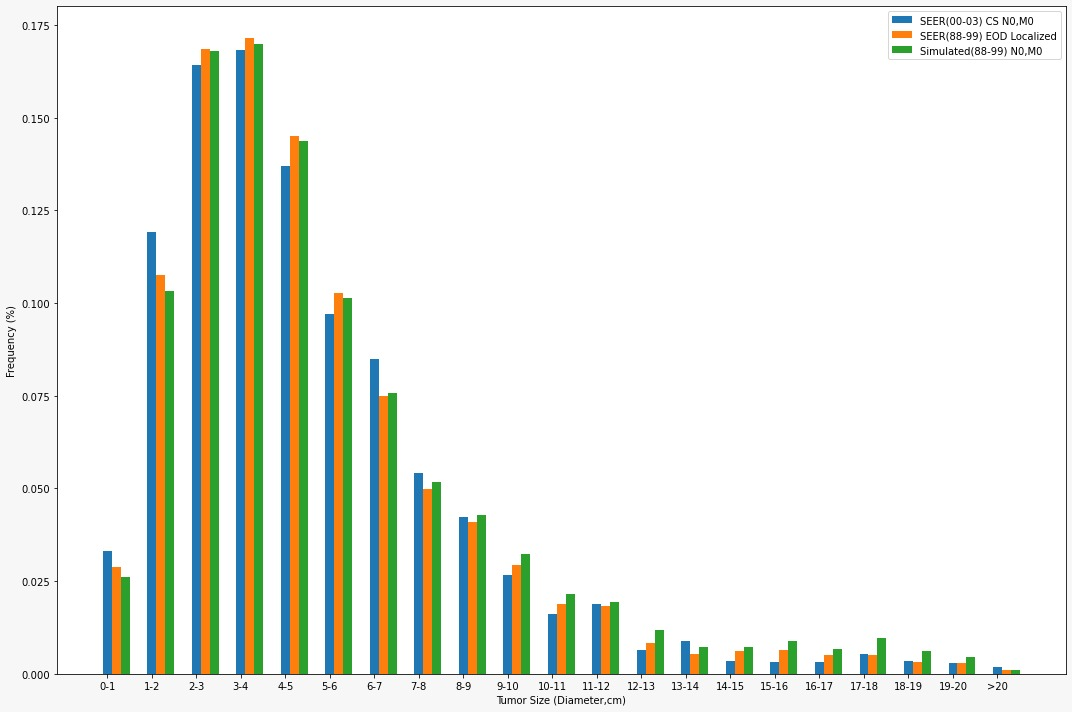
\includegraphics[scale=.2]{5.jpeg}}
		\caption{Stage N0,M0 in SEER (2004–2008) and model (1988–1999), stage Localized by SEER standard in SEER (1988–1999)
		}		
	\end{figure}	
	
	\begin{figure}[htbp]
		\centerline{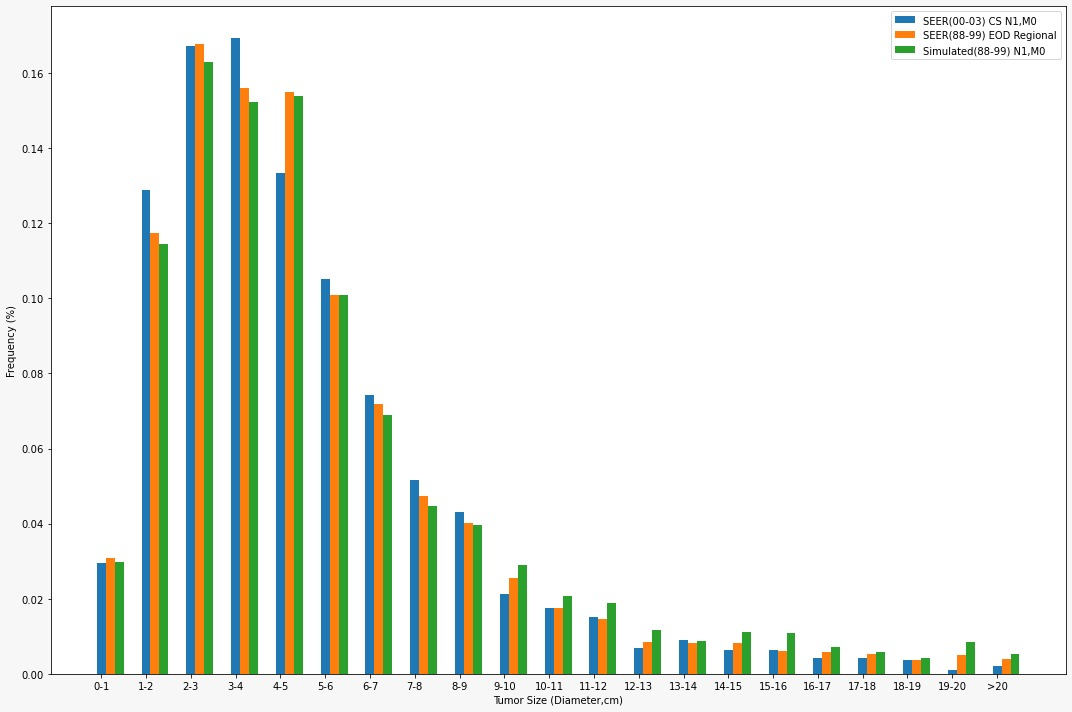
\includegraphics[scale=.2]{6.jpeg}}
		\caption{Stage Nx,M0 (x$>$=1) in SEER (2004–2008) and model (1988–1999), stage Regional by SEER standard in SEER (1988–1999)
		}		
	\end{figure}
The above graph shows comparison in characteristics of distribution N0,M0 staged patients based upon tumor size ranges, between SEER 2000-2003, SEER 1988-99 and simulations of SEER 1988-99 based upon the model. The graph shows approximate convergence of SEER 1988-1999 and simulated SEER 1988-99 data on lung cancer patients distribution at some tumor size ranges, specifically in the initial ranges of tumor sizes. In some of the mid-ranges, one can also infer that the closeness in characteristics between 2000-2003 SEER data and prediction through simulated 1988-99 data.

\item  \textbf{\underline{Inferences from innovation}}

As we calculated the p-value which comes out to be 0.7903833203340546 for the dataset that we used for this test we can say that the p-value is significantly greater than the value of alpha which is 0.05 as we are estimating this test at a 95\% confidence interval. As the p-value is significantly greater ( $>>$0.05) hence there is strong evidence in the favour of  Null hypothesis so here we fail to reject the null hypothesis and thus, the districts with a high Genetic Risk have high lung cancer incidence rates than those with low genetic risk.
		
\item  \textbf{\underline{Inferences from Machine Learning Models}}

	\begin{figure}[htbp]
	\centerline{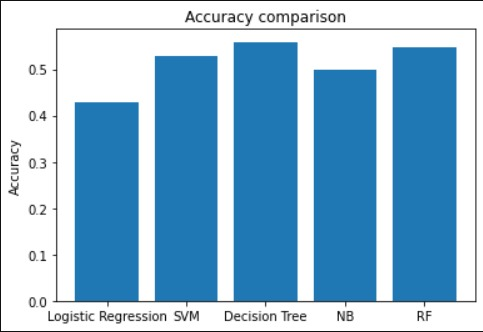
\includegraphics[scale=.35]{8.png}}
	\caption{Plot of accuracy comparison of different models
	}		
\end{figure}

We have implemented different types of modelling like Logistic regression classification, SVM (Support Vector Machine) classification ,Naive bayes classification , Decision tree classification , Random forest classification with the help of Machine Learning algorithms. And from that we have derived accuracy of that modelling on our dataset as a result. 


		
	\end{enumerate} 
	
	
	
	
	
	%\vspace{0.5cm}
	
\pagebreak
	
	\bibliographystyle{IEEEtran}
	\bibliography{ref.bib}
	\begin{enumerate}
		\item R. Bartoszyński et al., “Modeling cancer detection: tumor size as a source of information on unobservable stages of carcinogenesis,” Mathematical Biosciences, vol. 171, no. 2, pp. 113–142, Jun. 2001, doi: 10.1016/s0025-5564(01)00058-x.
		
		\item J. Malhotra, M. Malvezzi, E. Negri, C. La Vecchia, and P. Boffetta, “Risk factors for lung cancer worldwide,” Eur Respir J, vol. 48, no. 3, pp. 889–902, May 2016, doi: 10.1183/13993003.00359-2016.
		
		\item Mainakchaudhuri, “Lungs Cancer Classification and Data Analysis,” Kaggle, 04-Aug-2020. [Online]. Available: https://www.kaggle.com/mainakchaudhuri/lungs-cancer-classification-and-data-analysis. 
		\item Yasminehemmati, “Lung Cancer vs Air Quality,” Kaggle, 24-Sep-2020. [Online]. Available: https://www.kaggle.com/yasminehemmati/lung-cancer-vs-air-quality.
		
    	\item M. D. Lynne Eldridge, “Is Lung Cancer Genetic?,” Verywell Health, 01-Apr-2021. [Online]. Available: https://www.verywellhealth.com/is-lung-cancer-inherited-2248975#:~:text=1 It has been estimated,in your family has it.
    	
    	\item M. Acharjee, K. P. Das, and Y. S.Stanley, “Air Quality-Lung Cancer Data,” Harvard Dataverse, 31-Jan-2020. [Online]. Available: https://dataverse.harvard.edu/dataset.xhtml?persistentId=doi:10.7910/DVN/HMOEJO. 
	\end{enumerate}
	
\end{document}